\chapter{Background}\label{ch:chapter2} % For referencing the chapter elsewhere, use \ref{Chapter1}
%
%%----------------------------------------------------------------------------------------
%
To start with, we bring up what is video coding, why it is needed, and
its challenges.
Next we discuss what is deep learning, the history of deep learning and how
it works for vision tasks.
Furthermore, we introduce how we plan to apply deep learning to optimize video
coding tasks and why it should work.
In the end, a survey of related works in video coding and deep learning is given.

%3D Video applications are attracting more interests
%%----------------------------------------------------------------------------------------
%
\section{Video Coding}\label{sec:video-coding}
Video playback is the most straightforward way for human to perceive dynamic
scenes that exist across a time series.
More than half of the neurons in human brain are born to process the visual
information which is supplied by human eyes.
It becomes effortless for human to understand things presented by
the video playback instead of a long paragraph of words.
Videos are made up of consecutive sets of image frames, which in turn
are made up of pixel matrices.
Visual information of a cosmic scale is first stored by various methods
then delivered during a period of video playback.

In 1950s, video tapes were employed to store the videos.
Video tape is able to serve for about eight to twelve years
before the video quality starts to degrade.
In 1970s, laser disc appeared in the US market as an alternative of video tapes.
Start from laser disc, the video storage started its new era in digital world.
In 1990s, DVDs were released after laser disc.
Data is stored in spiralling tracks on the disc.
A laser beam can be utilized to read the data.
In addition, hard drives, flash drives and SD cards were also starting to
become popular in the late 90s.
Nowadays, the cloud storage is very common in daily lives.
It is capable of storing data on the servers which are
accessible from any devices via internet connections.

Although so many formats are available for video storage, they share a common
feature: the more storage you use, the more cost it will be.
Let's take the cloud storage as an example.
Google cloud is one of the most popular cloud services in our daily lives.
It provides cloud storage with a price
of \$0.026 per GB/month~\parencite{RN202}
(this price is observed on 21 Nov 2017, it may change in the future).
If a 4K video with a resolution of 4096*2160,
at 120 frames per second,
8 bits for each of the RGB component, needs to be stored without
any compression in Google cloud,
we need to pay a monthly fee:
\((4096*2160*120*60*90*3*0.026)/(1024*1024*1024) \approx 416.47\) \$.
Without doubt, this figure is relatively not acceptable for just
storing the video.
High compression is needed to store the videos in a practical way.

From the other perspective, let us take the bandwidth into consideration.
To deliver the uncompressed 4K video which has been mentioned in
the previous paragraph, we need a bandwidth of:
\((4096*2160*120*3)/(1024*1024*1024) \approx 2.97\) Gigabytes per second.
The maximum bandwidth of Wireless 802.11ac, which is one of the common
internet access technologies, is 1.3 Gigabytes per second~\parencite{RN203}.
Apparently, the wireless connection is not able to deliver such kind of
4K videos.
High compression is desired to deliver the video through the internet.

Despite the fact that raw videos usually contain a large amount of data,
a lot of redundancies exist.
For every video sequence, two types of redundancies are ubiquitous: Spacial
Redundancy and Temporal Redundancy.
Video coding technologies are taking advantages of those redundancies to
achieve the efficient compression for video data.
Many of the useful video coding technologies have been adopted by the
international video coding standards, such as MPEG-4, H.264, H.265, etc.

Figure~\ref{fig:video-std-brief-history} shows the brief history of the
video coding standards.
\begin{figure}
    \centering
    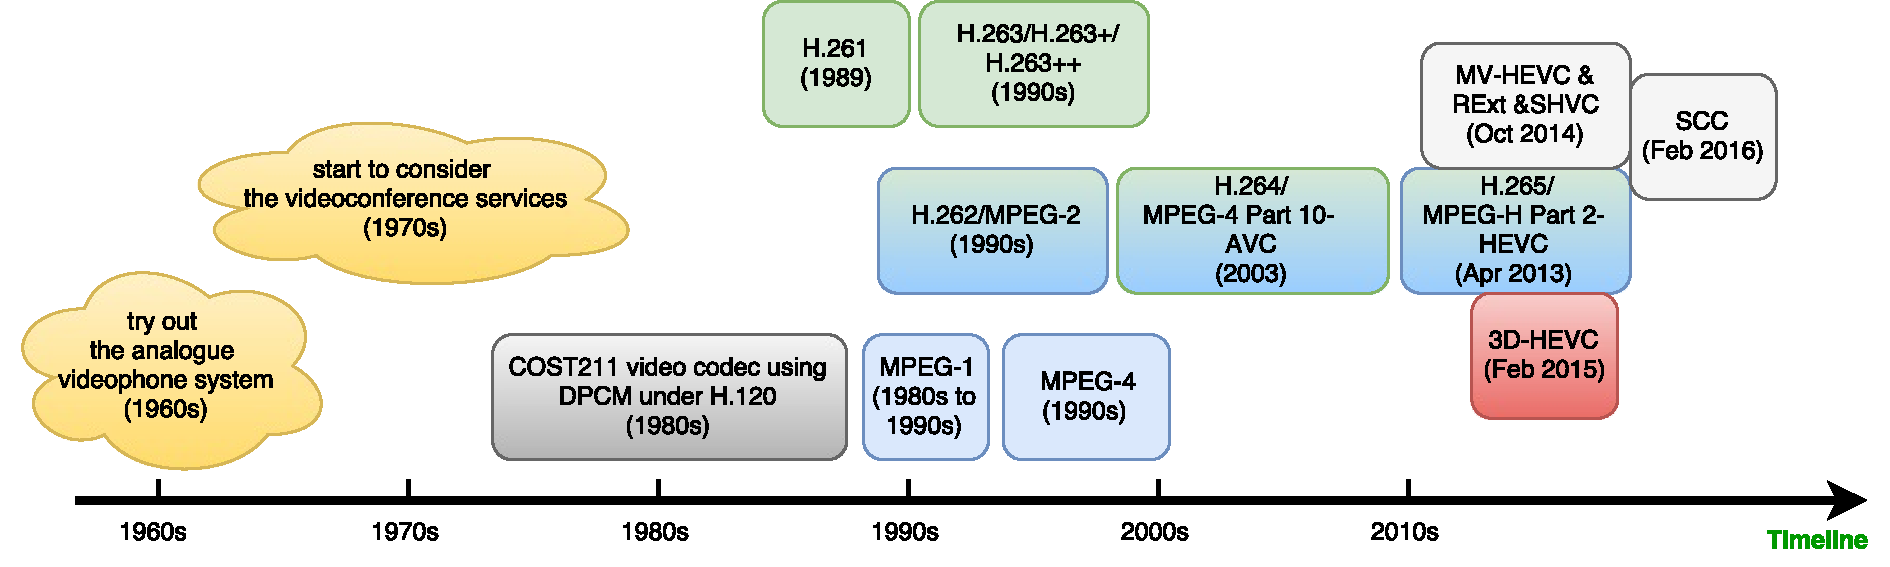
\includegraphics[width=\textwidth,height=\textheight,keepaspectratio]{Figures/video-std-brief-history.pdf}
%        \decoRule
    \caption[The brief history of the video coding standards]
    {The brief history of the video coding standards}
    \label{fig:video-std-brief-history}
\end{figure}
In 1980s, the COST211 video codec, built on top of Differential
Pulse Code Modulation (DPCM), was standardized under H.120 standard by CCITT
(now known as ITU-T).
In late 1989, the H.261 was completed and its success marked a milestone for
video coding at low bit rate with fairly good quality~\parencite{RN181}.
The Motion Picture Experts Group (MPEG) kicked off the exploration of video
storage, such as CD-ROMs.
Their objective was to achieve a competitive performance with cassette
recorders in terms of compression of videos which have rich motions.
The framework of H.261 had been used to start the codec design of MPEG-1.
MPEG-2 was one generation after the MPEG-1.
It featured higher capabilities when handling videos with
high bit rates and high resolutions.
In MPEG-2, the encoder is allowed to make its own decision on the
the number of bi-directionally predicted pictures according to a
suitable coding delay.
ITU-T found this technique applicable to telecommunication applications, as
a result MPEG-2 has been adopted as H.262 for telecommunications.
Right after the MPEG-2 standard, MPEG-3 was designed mainly for coding of
high definition videos.
However, MPEG-3 was discarded due to the versatility of MPEG-2, which
can be used to encode videos of any resolutions.
In the late 1998, MPEG-4 was introduced as a way of defining compression of
both audio and visual digital data.
Later on MPEG-4 was divided into several parts during its continuously evolving.
Among its sub-parts, MPEG-4 part 10 (a.k.a. Advanced Video Coding) is mainly
for the video compression.
With the rising popularity of the high definition videos, the new standard
termed High Efficiency Video Coding (HEVC) for compressing videos in a more
efficient way comparing with previous standards, such as H.264/AVC, has
emerged under the efforts from the Joint Collaborative Team on Video
Coding (JCT-VC).
In the meanwhile, five extensions of the HEVC standard, comprising
Format Range Extension (RExt), Scalability Extension (SHVC),
Multi-view Extension (MV-HEVC), 3D Extension (3D-HEVC),
Screen Content Coding Extension (SCC),  have been finalized
from 2014 to 2016 to fulfill extra requirements in various video coding
scenarios.

In this work, we focus on the depth map coding in 3D-HEVC\@.
The 35 angular modes and depth modeling modes have been embraced in the
depth map coding tools in 3D-HEVC\@.
The DMM1 mode introduces an huge increase for the encoding time of 3D videos.
Acceleration of the depth map coding is needed.

\section{Deep Learning}\label{sec:deep-learning}
Deep learning is an approach of representation learning
(a.k.a. feature learning), which is essentially a method to
learn from data.
Numerous layers of computational units together with appropriate activating
mechanism comprise the basic architecture for deep learning.
Multitudinous data sets are needed for those computational architectures
to learn data abstractions
for tasks such as image classification, speech recognition,
object detection, etc.
Each layer learns a level of abstraction from the data sets using
back-propagation algorithm~\parencite{RN96}.
Making use of those learned abstractions, the computational architectures are
able to solve complex problems which are typically non-linear and normally hard
to solve by using specific rules that are designed in advance.

Deep learning has been attracting wide attention from all over the world
in recent years, not only because of the great achievements it has
made in various application scenarios, but also due to the promise of an
intelligent future it gives.
Such a learning methodology makes people believe it is possible
for the formation of wise machines
that they have long dreamed to possess.
The growing data accessibility provides rich examples for deep computational
architectures to adjust their internal weights and bias until their
predictions have low error rate.
On the other hand, the computational devices are relatively
affordable than in the previous years by the society, with the help of which,
accelerations of learning processes has been achieved, hence a bunch of
time consuming deep learning architectures can be tried within acceptable
periods.

In the ILSVRC-2012 competition~\parencite{RN205}, AlexNet~\parencite{RN65}
received the championship with the 15.3\% top-5 error rate, compared to
26.2\% achieved by the runner-up.
Such a large margin of error rate claimed a breakthrough in
object recognition history.
It kicked off a blistering pace of trying out deep learning by both academia
and industry, which in turn led to an increase of the convolutional
neural networks' submissions to ILSVRC-2013, in which ZF Net~\parencite{RN66}
was the winner.
It fine-turned the architecture of AlexNet based on the
gorgeous visualizations of trained models.
Both AlexNet and ZF Net are of the same structure which is built up
by simply stacking computational layers while GoogLeNet~\parencite{RN60}
is composed of Inception
modules.
This new architecture was the most successful candidate in ILSVRC-2014.
It has not only set the new height of object recognition but also started to
optimize the computational resources of the network by design.
It consists of 22 layers, which was deeper than all the previous
networks in ILSVRC\@.
However, it is still not deep enough.
In ILSVRC-2015, Residual Neural Network (ResNet)~\parencite{RN67} with
152 layers won the championships in all the five main tracks.
ResNet introduced a brand new notion into the neural network architecture
named identity mapping.
The shortcut connection in the identity mapping prevents the degradation of
training accuracy when the network goes deeper.
Besides, the converging speed of ResNet is faster than the network built up
with Inception modules when both are of the similar size.

Despite the fact that neural networks built up from Inception modules
converge slower than those built up from ResNet modules, it is still
worth it for a brief review of the valuable insights residing in
the Inception networks.
A typical incarnation of the first generation of Inception networks is named
GoogLeNet~\parencite{RN60}.
It was intricately carved with a responsibility to win computer vision
tasks in ILSVRC-2014, on which it performed better than all the other
deep neural network architectures.
There exist philosophical reflections which are intend to serve as guidelines
for the construction of Inception networks.
Two major downsides of a enlarged neural network have been discussed
in~\parencite{RN60}.
One is the higher chances of overfitting while the other is
the strikingly increased requirements of computational resources with the
enlarged network size.
For handling those drawbacks, based on the new ideas which were introduced
in~\parencite{RN207} about how to construct the reasonable architecture of
neural networks, new experiments orienting sparse network structure have
been tried out.
One year later after GoogleNet hold the championship of ILSVRC-2014,
a method named Batch Normalization~\parencite{RN61} has been
proposed by Google researchers to accelerate and ease the
training of deep neural networks.
The core idea behind Batch Normalization is to normalize
the inputs to each layer for every batch of training data.
More importantly, based on the observation that the normalization process
essentially is matrix multiplications followed by adding biases, the Batch
Normalization is implemented as additional layers which makes it part of
the network architecture.
This fairly novel method started a new chapter for the training of deep
neural networks.
With the adoption of Batch Normalization, higher learning rates no longer
impede the convergence of the deep networks, oppositely faster
training speed is brought to scene which can achieve a
better accuracy of prediction with considerably less time.
Additionally, in some cases, it can even replace the Dropout~\parencite{RN70}
which is an effective method to prevent overfitting.
The incorporation of Batch Normalization into the first generation of
Inception network architecture led to the formation of Inception-v2, which
improved the best accuracy on ImageNet classification with less training steps.
%more advanced accuracy on ILSVRC 2012
%classification challenge validation set.
In the same year, Inception-v3~\parencite{RN62} joined the party, the objective of which was
to effectively leverage the power of additional computation by factorizing
to smaller size convolutions and regularizing the classifier layer with
the estimation of minor effect of label-dropout in the training process.
The network architectures were scaled up in Inception-v3, which consequently
imposed higher requirements of available computational resources.
With the ResNet~\parencite{RN67} stealing the show in ILSVRC-2015,
the influence of the
identity connections in residual units on the learning process
has been investigated in~\parencite{RN63}.
The filter concatenation stage of in Inception-v3 is replaced using identify
connections which led to the layout of a new model named Inception-ResNet-v1.
A more advanced version which was named Inception-ResNet-v2 has a larger
network size than the first version.
Besides the mixed architectures of Inception-ResNet, a pure Inception
incarnation named Inception-v4 was also presented with comparison to
Inception-ResNet-v2.
Both Inception-v4 and Inception-ResNet-v2 have significant gain of performance
mainly benefiting from the enlarged size of network.

\section{Related Work}\label{sec:related-work}
In this section, the prior arts on optimizations for video
coding are reviewed.
Before the finalization of 3D-HEVC standard in Feb 2015, a lot of works on
depth map have been published mainly focusing on improving the coding
performance of depth map.
%Although in this thesis the researching focus is 3D-HEVC oriented, it is
%still helpful to know the related works in HEVC\@.
%We start with a review of fast intra coding for HEVC,
%after that fast depth coding for 3D-HEVC\@.
%\subsection{Fast Intra Coding in HEVC}\label{subsec:fast-HEVC}
%
%\subsection{Fast depth Coding in 3D-HEVC}\label{subsec:fast-3D-HEVC}
Based on the observation that the depth map is characterized by vast
smooth regions separated by sharp edges, an algorithm to effectively
encode homogeneous regions has been proposed in~\parencite{RN120}.
It improves coding performance for depth maps by copying pixel values for
homogeneous blocks from values of neighboring reference pixels.
In~\parencite{RN123}, Depth Lookup Table (DLT) has been proposed for
encoding the depth maps in 3D-HEVC standard.
It offers the benefits of 1.3\% bit-rate reduction.
To further improve the coding performance for depth map, more
dedicated tools for depth map coding are needed.
Depth Modeling Modes (DMM) and View Synthesis Optimization (VSO) are proposed
in~\parencite{RN208}.
VSO provides 17\% bit rate reduction in average while DMM provides 6\% savings
on bit rate.
Although the introduction of DMM and VSO have brought the coding performance of
depth map coding into a new level, the computational complexity has increased
a lot due to the complex nature of VSO\@.
Consequently the time cost of depth map encoding becomes fairly expensive.
This raised the question of whether it is possible to reduce the computational
complexity for saving encoding time.
In~\parencite{RN76}, a fast wedgelet searching scheme achieves significant
reduction for computational complexity with minor BD-rate increase.
It takes advantage of the result from
Sum of Absolute Transform Difference (SATD) to reduce the wedgelet searching
candidates.
Rough RD cost from Rough Mode Decision is used as mode selection threshold
in~\parencite{RN90} to speed up the Bi-partition modes decision.
A two-step fast searching approach for wedgelet partition
appears in~\parencite{RN126}.
It features a coarse search in conjunction with a further refinement step.
Another fast approach for wedgelet searching~\parencite{RN79}
is to make use of the Most Probable Mode (MPM) to reduce wedgelet
searching candidates.
Since intra angular modes will lead to ringing artifacts
when utilized for depth map coding, the idea of skipping intra
angular prediction by making use of edge detector is shown in~\parencite{RN89}.
Bayesian classifier is used in~\parencite{RN102} to alleviate the computational
complexity of intra mode decision in 3D-HEVC\@.

After the finalization of 3D-HEVC, a lot of algorithms has been proposed
to accelerate depth map encoding.
The optimal mode of the parent prediction unit (PU)
in the hierarchical quad-tree coding structure has been utilized to select
the mode for child prediction unit (PU) in~\parencite{RN131}, and early
decision for segment-wise DC coding is used together to achieve faster
depth intra coding.
Edge classification in Hadamard transform domain is used in~\parencite{RN86}
to skip the DMM decision process conditionally.
The minimum RD cost of the candidates in the full-RD searching list is taken
as a threshold to bypass DMM decision based on the comparisons with the
header rates in~\parencite{RN93}.
Most probable region for DMM1 mode decision is identified with the help
of sharp edges in~\parencite{RN209}, and DMM3 is skipped when depth
prediction unit (PU) does not match with co-located texture counterpart.
Variance is utilized in~\parencite{RN210} to estimate the most promising
sub-region for DMM1.
Corner point is used for fast quad-tree decision of depth intra coding
in~\parencite{RN211}.
Variance distribution is studied in~\parencite{RN111}, based on which the
method termed Squared Euclidean distance of variances (SEDV) is
proposed to substitute the long-standing View Synthesis Optimization (VSO)
process.
Besides, a new scheme termed probability-based early depth intra mode
decision (PBED) is employed to skip modes and the RD cost in
Rough Mode Decision (RMD) is used to terminate
segment-wise depth coding (SDC)~\parencite{RN123}
as early as possible.
The correlation between depth maps and texture views are explored
in~\parencite{RN94} to alleviate the complexity of the
compression for depth map.
In~\parencite{RN212}, comparing RD cost with pre-calculated threshold for fast
intra mode decision together with early decision for the CU depth are used
to accelerate the encoding process.
Making use of RD cost results of the angular modes, only the most promising
DMMs are evaluated in~\parencite{RN87} and, moreover, an innovative
method using golden ratio to further improve the
depth map coding is proposed.
The characteristics of depth map are studied in~\parencite{RN91},
as a result only four conventional intra modes are used for
depth map intra coding and only six directions are used in DMM1 searching.
Block edge along with the border gradient are used together
in~\parencite{RN114} to accelerate the depth map coding.
Information of neighbouring blocks and threshold which is derived from
lots of experiments are used in~\parencite{RN85} for improving depth
map coding.

In~\parencite{RN74}, the decision for the depth of the coding unit
in High Efficiency Video Coding (HEVC) is modeled as a classification
problem which is solved by machine learning approach.
A shallow convolutional neural network (CNN) is
used in~\parencite{RN78} to determine coding unit depth in
High Efficiency Video Coding (HEVC) while
in~\parencite{DBLP:journals-corr-abs-1710-01218}, a deeper convolutional
neural network together with long- and short-term memory (LSTM) network
are employed to address the same issue.
In additional to the works which are targeting the
coding unit depth decision using machine learning approaches, it is found
in~\parencite{RN73} that deep learning is used for the intra mode
selection in High Efficiency Video Coding (HEVC).
%Since the angular modes are designed for preserving texture
%patterns, it does not work well on keeping the fidelity of depth maps.
%Simply using angular mode to encode depth maps,
%inging artifacts~\parencite{RN44} occur in the sharp edges on depth maps
%which tend to cause distortions on synthesized views.
%Depth maps are not directly presented to audience while synthesized views are.
%Apparently attention is needed for improvements.

% ====== can be used for literature review =====
%AlexNet contains five convolutional layers and three fully-connected
%layers.
%The Rectified Linear Units (ReLU)~\parencite{RN206}, Local Response
%Normalization and Overlapping Pooling were adopted.
%The methodology of multiple GPU training was used to make the learning fast.
%Data Augmentation and Dropout were chosen to overcome the problem of
%Overfitting.
%Stochastic gradient descent was adopted.
% ====== can be used for literature review =====




%Welcome to this \LaTeX{} Thesis Template, a beautiful and easy to use template for writing a thesis using the \LaTeX{} typesetting system.
%
%If you are writing a thesis (or will be in the future) and its subject is technical or mathematical (though it doesn't have to be), then creating it in \LaTeX{} is highly recommended as a way to make sure you can just get down to the essential writing without having to worry over formatting or wasting time arguing with your word processor.
%
%\LaTeX{} is easily able to~\parencite{RN93} professionally typeset documents that run to hundreds or thousands of pages long. With simple mark-up commands, it automatically sets out the table of contents, margins, page headers and footers and keeps the formatting consistent and beautiful. One of its main strengths is the way it can easily typeset mathematics, even \emph{heavy} mathematics. Even if those equations are the most horribly twisted and most difficult mathematical problems that can only be solved on a super-computer, you can at least count on \LaTeX{} to make them look stunning.
%
%%----------------------------------------------------------------------------------------
%
%\section{Welcome and Thanku}\label{sec:welome}
%Welcome to this \LaTeX{} Thesis Template, a beautiful and easy to use template for writing a thesis using the \LaTeX{} typesetting system.
%
%If you are writing a thesis (or will be in the future) and its subject is technical or mathematical (though it doesn't have to be), then creating it in \LaTeX{} is highly recommended as a way to make sure you can just get down to the essential writing without having to worry over formatting or wasting time arguing with your word processor.
%
%\LaTeX{} is easily able to professionally typeset documents that run to hundreds or thousands of pages long. With simple mark-up commands, it automatically sets out the table of contents, margins, page headers and footers and keeps the formatting consistent and beautiful. One of its main strengths is the way it can easily typeset mathematics, even \emph{heavy} mathematics. Even if those equations are the most horribly twisted and most difficult mathematical problems that can only be solved on a super-computer, you can at least count on \LaTeX{} to make them look stunning.
%
%%----------------------------------------------------------------------------------------
%
%\section{Welcome and ThYou}\label{sec:weome}
%Welcome to this \LaTeX{} Thesis Template~\parencite{Reference1}, a beautiful and easy to use template for writing a thesis using the \LaTeX{} typesetting system.
%
%If you are writing a thesis (or will be in the future) and its subject is technical or mathematical (though it doesn't have to be), then creating it in \LaTeX{} is highly recommended as a way to make sure you can just get down to the essential writing without having to worry over formatting or wasting time arguing with your word processor.
%
%\LaTeX{} is easily able to professionally typeset documents that run to hundreds or thousands of pages long. With simple mark-up commands, it automatically sets out the table of contents, margins, page headers and footers and keeps the formatting consistent and beautiful. One of its main strengths is the way it can easily typeset mathematics, even \emph{heavy} mathematics. Even if those equations are the most horribly twisted and most difficult mathematical problems that can only be solved on a super-computer, you can at least count on \LaTeX{} to make them look stunning.
%
%%----------------------------------------------------------------------------------------
%
%\section{Welcome and Thau}\label{sec:welcoe}
%Welcome to this \LaTeX{} Thesis Template, a beautiful and easy to use template for writing a thesis using the \LaTeX{} typesetting system.
%
%If you are
%\begin{table}
%
%    \label{tab:treatments}
%    \centering
%%    \begin{tabular}{l l l}
%%        \toprule
%%        \tabhead{Groups} & \tabhead{Treatment X} & \tabhead{Treatment Y} \\
%%        \midrule
%%        1 & 0.2 & 0.8\\
%%        2 & 0.17 & 0.7\\
%%        3 & 0.24 & 0.75\\
%%        4 & 0.68 & 0.3\\
%%        \bottomrule\\
%%    \end{tabular}
%    \begin{tabular}{c r @{.} l}
%        Pi expression       &
%        \multicolumn{2}{c}{Value} \\
%        \hline
%        $\pi$               & 3&1416  \\
%        $\pi^{\pi}$         & 36&46   \\
%        $(\pi^{\pi})^{\pi}$ & 80662&7 \\
%    \end{tabular}
%    \caption{The effects of treatments X and Y on the four groups studied.}
%\end{table}
%writing a thesis (or will be in the future) and its subject is technical or mathematical (though it doesn't have to be), then creating it in \LaTeX{} is highly recommended as a way to make sure you can just get down to the essential writing without having to worry over formatting or wasting time arguing with your word processor.
%
%\LaTeX{} is easily able to professionally typeset documents that run to hundreds or thousands of pages long. With simple mark-up commands, it automatically sets out the table of contents, margins, page headers and footers and keeps the formatting consistent and beautiful. One of its main strengths is the way it can easily typeset mathematics, even \emph{heavy} mathematics. Even if those equations are the most horribly twisted and most difficult mathematical problems that can only be solved on a super-computer, you can at least count on \LaTeX{} to make them look stunning.
%
%%----------------------------------------------------------------------------------------
%
%\section{Welcome and Tnk You}\label{sec:wlcome}
%Welcome to this \LaTeX{} Thesis Template, a beautiful and easy to use template for writing a thesis using the \LaTeX{} typesetting system.
%
%If you are writing a thesis.
%
%%\begin{verbatim}
%\begin{figure}
%    \centering
%    
\includegraphics{Figures/Electron}
%    %    \decoRule
%    \caption[An Electron]{An electron (artist's impression).}
%    \label{fig:Electron}
%\end{figure}
%%\end{verbatim}
%(or will be in the future) and its subject is technical or mathematical (though it doesn't have to be), then creating it in \LaTeX{} is highly recommended as a way to make sure you can just get down to the essential writing without having to worry over formatting or wasting time arguing with your word processor.
%
%\LaTeX{} is easily able to professionally typeset documents that run to hundreds or thousands of pages long. With simple mark-up commands, it automatically sets out the table of contents, margins, page headers and footers and keeps the formatting consistent and beautiful. One of its main strengths is the way it can easily typeset mathematics, even \emph{heavy} mathematics. Even if those equations are the most horribly twisted and most difficult mathematical problems that can only be solved on a super-computer, you can at least count on \LaTeX{} to make them look stunning.
%
%%----------------------------------------------------------------------------------------